\documentclass{beamer}

\usepackage[utf8]{inputenc}
\usepackage[T2A]{fontenc}
\usepackage[russian,english]{babel}
\usepackage{graphicx}
\usepackage{listings}

\usetheme{Madrid}
\setbeamertemplate{caption}{\raggedright\insertcaption\par}

\setbeamercolor{structure}{fg=blue}

\lstset{
	language=C,
	basicstyle=\ttfamily\tiny,
	keywordstyle=\color{blue},
	stringstyle=\color{red},
	commentstyle=\color{gray},
	showstringspaces=false,
	frame=single,
	breaklines=true,
	numbers=left,
	numberstyle=\tiny\color{gray}
}

\title{Бинарная система счисления}
\author[Какнаев А.В.]{Какнаев Артем Владимирович}
\institute[ИМИТ]{Институт математики и информационных технологий}
\date{Петрозаводск - 2026}


\AtBeginSection[]
{
	\begin{frame}
		\frametitle{Содержание}
		\tableofcontents[currentsection]
	\end{frame}
}

\begin{document}
	
	\begin{frame}
		\titlepage
	\end{frame}
	
	\begin{frame}
		\frametitle{Содержание}
		\tableofcontents
	\end{frame}
	
	\section{Введение}
	
	\begin{frame}
		\frametitle{Что такое бинарная система}
		
		Бинарная система счисления используется во всех современных компьютерах.
		
		\pause
		
		\begin{itemize}
			\item Использует только цифры 0 и 1
			
			\item Это основа хранения данных
			
			\item Применяется в процессорах и памяти
		\end{itemize}
		
		\begin{figure}
			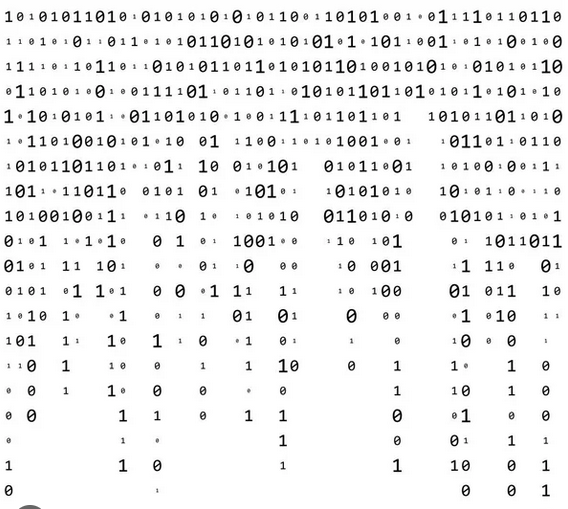
\includegraphics[width=0.5\textwidth]{binary.png}
			\caption{Двоичный код}
		\end{figure}
		
	\end{frame}
	
	\section{Основные понятия}
	
	\begin{frame}
		\frametitle{Определение}
		
		\textbf{Определение.}
		
		Бинарная система счисления — это позиционная система счисления с основанием 2.
		
		\pause
		
		В ней используются только две цифры:
		
		\[
		0 \quad \text{и} \quad 1
		\]
		
		\pause
		
		Любое число записывается как последовательность нулей и единиц, например:
		
		\[
		1011_2
		\]
		
	\end{frame}
	
	\begin{frame}
		\frametitle{Пример перевода числа}
		
		Переведём число 13 из десятичной системы в двоичную:
		
		\pause
		
		\[
		13_{10} = 1101_2
		\]
		
		\pause
		
		Проверка через разложение по степеням двойки:
		
		\[
		13 = 1 \cdot 2^3 + 1 \cdot 2^2 + 0 \cdot 2^1 + 1 \cdot 2^0
		\]
		
		\pause
		
		\[
		13 = 8 + 4 + 0 + 1 = 13
		\]
		
	\end{frame}
	
	\section{Математические основы}
	
	\begin{frame}
		\frametitle{Формула представления числа}
		
		Любое двоичное число можно представить в виде суммы:
		
		\begin{equation}
			N = \sum_{i=0}^{n} a_i \cdot 2^i
		\end{equation}
		
		\pause
		
		где:
		\begin{itemize}
			\item $a_i$ — это цифры 0 или 1
			\item $2^i$ — это степени двойки
			\item $n$ — количество разрядов минус 1
		\end{itemize}
		
	\end{frame}
	
	\begin{frame}
		\frametitle{Теорема}
		
		\textbf{Теорема.}
		
		Любое натуральное число можно единственным образом представить в виде суммы степеней двойки.
		
		\pause
		
		\textbf{Пример:}
		
		Возьмём число 25:
		
		\[
		25 = 16 + 8 + 1
		\]
		
		\pause
		
		В двоичной системе:
		
		\[
		25_{10} = 11001_2
		\]
		
		\pause
		
		Потому что:
		
		\begin{equation}
			25 = 1 \cdot 2^4 + 1 \cdot 2^3 + 0 \cdot 2^2 + 0 \cdot 2^1 + 1 \cdot 2^0
		\end{equation}
		
	\end{frame}
	
	\begin{frame}
		\frametitle{Алгоритм перевода делением}
		
		Второй способ перевода — делить число на 2 и записывать остатки.
		
		\pause
		
		\textbf{Пример:} переведём 13 в двоичную систему.
		
		\pause
		
		\begin{itemize}
			\item $13 \div 2 = 6$, остаток 1
			\pause
			\item $6 \div 2 = 3$, остаток 0
			\pause
			\item $3 \div 2 = 1$, остаток 1
			\pause
			\item $1 \div 2 = 0$, остаток 1
		\end{itemize}
		
		\pause
		
		Читаем остатки снизу вверх: 1101
		
		\pause
		
		\textbf{Ответ:} $13_{10} = 1101_2$
		
	\end{frame}
	
	\section{Применение}
	
	\begin{frame}
		\frametitle{Где применяется}
		
		Бинарная система используется везде в компьютерах:
		
		\pause
		
		\begin{enumerate}
			\item Компьютерные процессоры
			\pause
			\item Оперативная память
			\pause
			\item Жёсткие диски и SSD
			\pause
			\item Передача данных по сети
		\end{enumerate}
		
		\pause
		
		\begin{figure}
			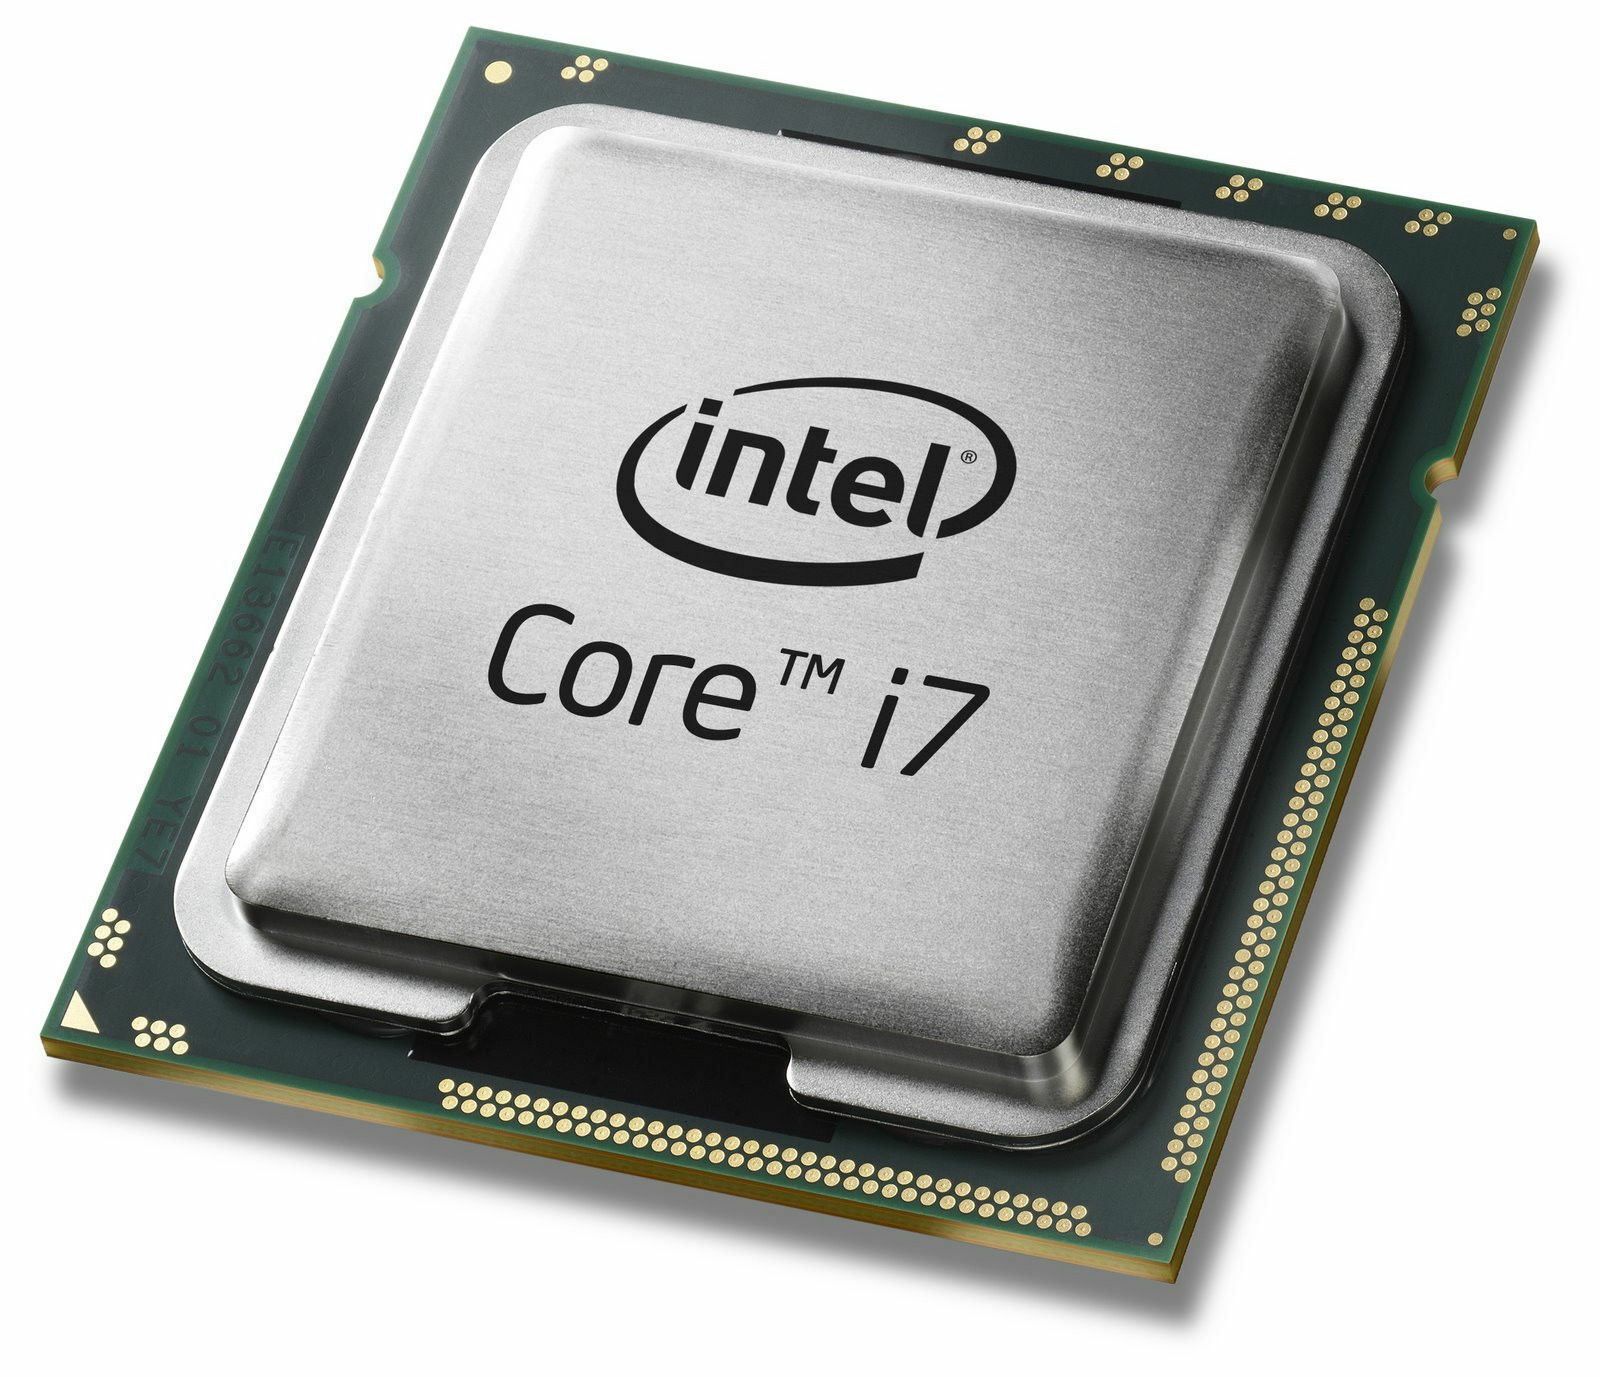
\includegraphics[width=0.4\textwidth]{image.png}
			\caption{Компьютерный процессор}
		\end{figure}
		
	\end{frame}
	
	\begin{frame}[fragile]
		\frametitle{Пример программы на C}
		
		Программа для вывода двоичного представления числа:
		
		\vspace{0.2cm}
		
		\begin{lstlisting}
			#include <stdio.h>
			
			void printBinary(int n) {
				for (int i = 7; i >= 0; i--) {
					printf("%d", (n >> i) & 1);
				}
				printf("\n");
			}
			
			int main() {
				int number = 10;
				printf("Chislo %d: ", number);
				printBinary(number);
				return 0;
			}
		\end{lstlisting}
		
		
	\end{frame}
	
	\section{Заключение}
	
	\begin{frame}
		\frametitle{Выводы}
		
		\begin{itemize}
			\item Бинарная система счисления является фундаментальной основой всей современной вычислительной техники
			\pause
			\item Все данные в компьютере (числа, текст, изображения, звук) хранятся и обрабатываются в виде последовательностей нулей и единиц
			\pause
			\item Теорема о единственности представления числа в двоичной системе гарантирует однозначность хранения и передачи информации
			\pause
			\item Понимание двоичной системы необходимо для изучения архитектуры компьютеров, программирования и криптографии
			\pause
			\item Алгоритмы перевода между системами счисления являются базовыми в информатике и используются повсеместно
		\end{itemize}
		
	\end{frame}
	
	\begin{frame}
		\frametitle{}
		
		
		\begin{center}
			\Huge Спасибо за внимание!
		\end{center}
		
	\end{frame}
	
\end{document}